%---------------------------------------------------------------------
%                          Cap�tulo 1
%---------------------------------------------------------------------
\chapter{Nombre del cap�tulo}
%Etiqueta del cap�tulo	
\label{}
%Estructura para poner una frase c�lebre
\begin{FraseCelebre}
\begin{Frase}
En la vida no existe nada que temer, \\
solo cosas que comprender.
\end{Frase}
\begin{Fuente}
Marie Curie
\end{Fuente}
\end{FraseCelebre}
%-------------------------------------------------------------------
%Aqu� empieza el cap�tulo 
\section{Introducci�n}
Contenido...
\subsection{Contenido...}
Contenido...
\subsubsection{Contenido..}
Contenido...
Ejemplo de cita \cite{RamPac20}.


\begin{figure}
	\centering
	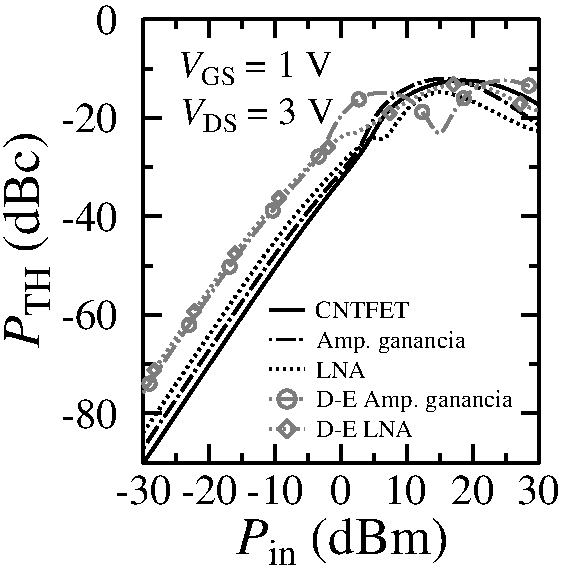
\includegraphics[width=0.45\linewidth]{fig/Capitulo1/Pin_ThirdHarmonic_es}
	\caption{Descripci�n de la figura.}
	\label{fig:pinthirdharmonices}
\end{figure}

Se recomienda al usuario de �sta plantilla utilizar figuras en formato PDF y para generar gr�ficas utilizar el software GLE, un script de ejemplo para generar la Figura \ref{fig:parametrossccamvds3vgs1cntfet} se puede encontrar dentro de la carpeta fig/FuentesCapitulo1.

\begin{figure}
	\centering
	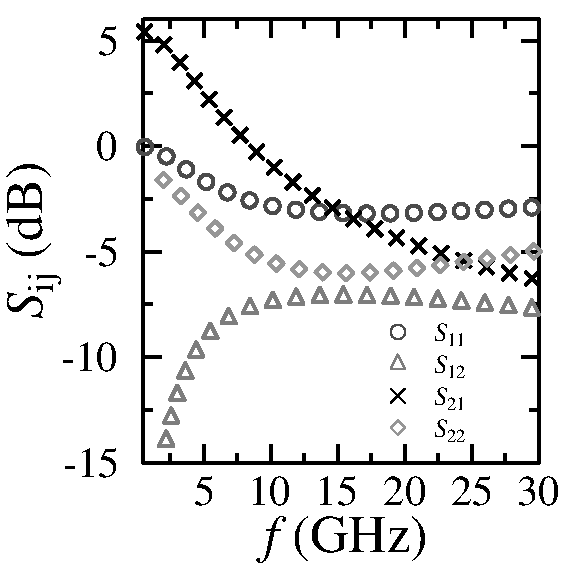
\includegraphics[width=0.45\linewidth]{fig/Capitulo1/Parametros_S_CCAM_VDS_3_VGS_1_CNTFET}
	\caption{Descripci�n de la figura.}
	\label{fig:parametrossccamvds3vgs1cntfet}
\end{figure}


%L�neas para a�adir la bibliograf�a por cada cap�tulo, utilizar bibtex.
\addcontentsline{toc}{chapter}{Referencias}
\printbibliography[segment=\therefsegment]


\endinput

